\chapter{Aproximación local de una función $\; \divideontimes$ }	

\section{Preliminares Introducción a las series de potencias}

Una \emph{serie de potencias} en torno al punto $x_0$ es una expresión del tipo:
\begin{equation}
	\label{serie-potencias}
	\sum _{ k=0 }^{ \infty }{a_n(x-x_0)^n}=a_0+a_1x+a_2x^2+a_3(x-x_0)^3\cdots 
\end{equation}

Donde $x$ es una variable y los coeficientes $a_n$ son constantes. Se dice que una serie de potencias `converge' en el punto $x=r$  si $\underset{N\to \infty}{lim }\;{\sum _{ k=0 }^{ N }{a_n(x-r)^n}}$ existe y es finito. En caso contrario se dice que la serie es divergente.

Obviamente, la serie de potencias \ref{serie-potencias} es convergente en $x=x_0$, ya que: 

$\sum _{ k=0 }^{ \infty }{a_n(x-x_0)^n}=a_0+0+0+\cdots =a_0$

	\begin{multicols}{2}
	Pero, ¿qué se puede decir de la convergencia de la serie \ref{serie-potencias} para otros valores de x?: las series de potencias convergen en un cierto intervalo de centro $x_0$ y diverge fuera de él. 

	Para cada serie de potencias existe un número $\rho; (0\le \rho \le \infty)$, llamado `radio de convergencia', de modo que la serie converge para $|x-x_0|<\rho$ y diverge para $|x-x_0|>\rho$. Si $\rho=\infty$, la serie de potencias converge para todo $\mathbb R$; si $\rho=0$, la serie solo converge en $x_0$.

	\begin{figure}[H]
		\centering
		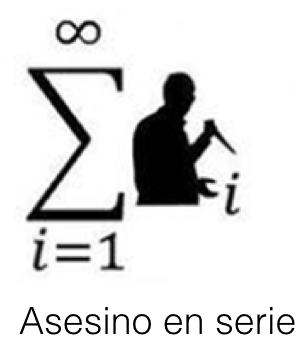
\includegraphics[width=0.25
	\textwidth]{imagenes/imagenes06/xiste06.png}
	\end{figure}
	\end{multicols}

Existen distintos \emph{criterios} para determinar si una serie es o no convergente y cual es su radio de convergencia, citamos, entre otros:
\begin{itemize}
	\item \emph{Criterio del cociente: } Si $\underset {n\to \infty}{lim}{\left| \dfrac {a_{n+1}}{a_n} \right|}=L$, donde $0\le L \le \infty$, entonces, el radio de convergencia de la serie de potencias $\sum _{ k=0 }^{ \infty }{a_n(x-x_0)^n}$ es $\rho=\dfrac 1 L$. con $\rho=\infty \leftrightarrow L=0 \quad \wedge \quad \rho=0 \leftrightarrow L=\infty$.
	
	Si este límite no existe, no podemos asegurar nada., hay que usar otros criterios.
	\item \emph{Criterio de la raíz: } Si $\underset{n\to \infty}{lim}{\sqrt[n]{|a_n|}}=L$,  con  $ 0\le L \le \infty$, entonces, el radio de convergencia de la serie de potencias $\sum _{ k=0 }^{ \infty }{a_n(x-x_0)^n}$ es, también  $\rho=1/L$, con las mismas observaciones anteriores.
\end{itemize} 

\section{Introducción a los desarrollos de Taylor y MacLaurin}

Puesto que este tema excede del temario usual de un curso de segundo de bachillerato, se ha optado por hacer su exposición más sencilla (no en la forma usual definiciones-teoremas) aún perdiendo un poco el rigor matemático en favor de la facilidad expositiva.

En este tema estudiaremos la aproximación de una función $f(x)$ en un entorno de un punto de su dominio, $a$ (`aproximación local') mediante funciones polinómicas $g(x)$ \emph{osculatrices}, es decir, tales de $f(a)=g(a); \; f'(a)=g'(a); \; f''(a)=g''(a); \; \cdots  ; \; f^{n)}(a)=g^{n)}(a)$.

Para la obtención de estas funciones deduciremos las fórmulas de \emph{Taylor} y \emph{MacLaurin} y estudiaremos las aplicaciones de estos desarrollos al cálculo de límites y determinación de extremos e inflexiones.

Aproximada una función pos estos métodos, el cálculo del valor de una función en un punto, $f(x)$, se simplifica enormemente al tener que calcular el valor de un polinomio en ese punto $g(x)$. Evidentemente se comete un error al hacer tal sustitución que dependerá del punto donde se realiza el cálculo, de la función que tengamos y del orden del polinomio que tomemos para hacer la sustitución de $f(x)$ por $g(x)$.


	\begin{figure}[]
		\centering
		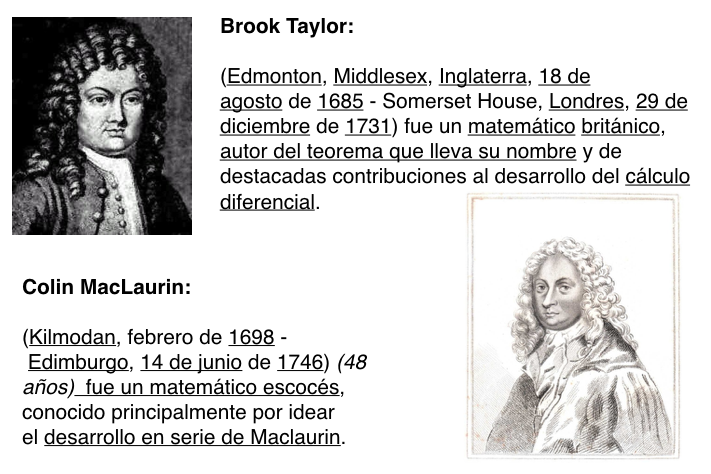
\includegraphics[width=1\textwidth]{imagenes/imagenes06/T06IM01.png}
		\caption{Taylor y MacLaurin.}
	\end{figure}
	
	\begin{multicols}{2}
	El problema de la aproximación local de una función real de variable real $f(x)$ en un punto $a 	\in  D(f)$ consiste en hallar otra función real de variable real $g(x)$ cuyos valores se diferencien `lo menos posible' de los de $f(x)$ en un entorno de $a$, así como conocer una cota del error cometido en tal sustitución ($f$ por $g$).
	\begin{figure}[H]
		\centering
		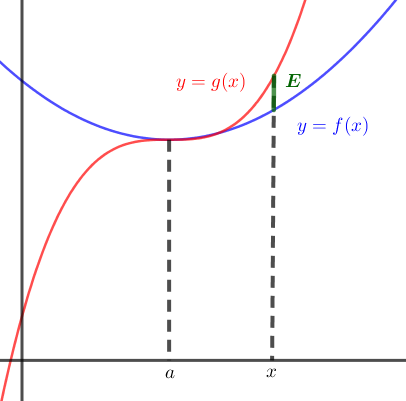
\includegraphics[width=0.25\textwidth]{imagenes/imagenes06/T06IM02.png}
	\end{figure}
	\end{multicols}
	
	En general, las funciones $g(x)$ más sencillas que resuelven estos problemas son los polinomios \textcolor{gris}{(fáciles de calcular para cualquier valor, de derivar, de integrar, ...)} Para obtenerlas deduciremos la ``Fórmula de Taylor''.
	
	\begin{figure}[H]
		\centering
		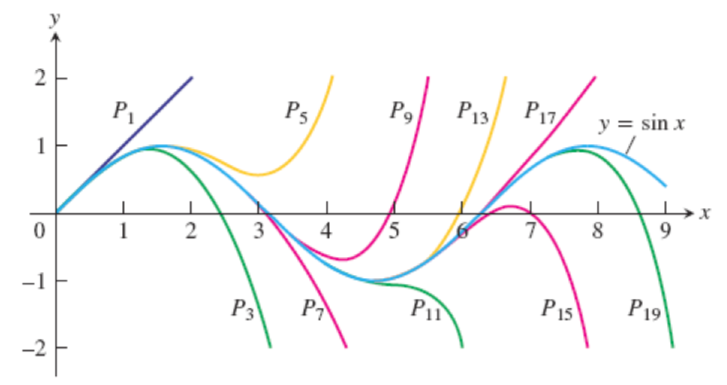
\includegraphics[width=1\textwidth]{imagenes/imagenes06/T06IM06.png}
		\caption{Aproximaciones de $\sin x$ con polinomios osculatrices.}
	\end{figure}
	
	\section{Fórmula de Taylor para funciones polinómicas}
	
	Sabemos que $\left( \mathcal{P}(x), +, \cdot\right)$, (donde  $\mathcal{P}(x)$ es el conjunto de los polinomios de una variable real) tiene estructura de `espacio vectorial'. El conjunto $\left\{1, (x-a),(x-a)^2,(x-a)^3,\cdots \right\}$ forma una base de $\mathcal{P}(x)$, por ello, cualquier polinomio se podrá expresar de forma única en esta base:
	
	$p(x)=a_0+a_1(x-a)+a_2(x-a)^2+a_3(x-a)^3+\cdots +a_n(x-a)^n$ (*)
	
	Veamos ahora si descubrimos que relación hay entre los coeficientes del polinomio $a_i$ y las derivadas sucesivas de $p(x)$ en $x=a$:
	
	$p(x)=a_0+a_1(x-a)+a_2(x-a)^2+\cdots +a_n(x-a)^n \to p(a)=a_0$
	
	$p'(x)=a_1+2a_2(x-a)+3a_3(x-a)^2+\cdots +n a_n(x-a)^{n-1} \to p'(a)=a_1$
	
	$p''(x)=2a_2+3\cdot 2 a3 (x-a)+ \cdots + n(n-1)a_n(x-a)^{n-2} \to p''(a)=2!\; a_2$
	
	$p'''(x)=3\cdot 2 a_3+ \cdots + n(n-1)(n-2)a_n (x-a)^{n-3}\to p'''(a)=3!\; a_3$
	
	$\cdots \cdots \cdots \cdots \cdots \cdots \cdots$
	
	$p^{n)}(x)=n(n-1)(n-2)(n.3)\cdots 3\cdot 2 a_n \to p^{n)}(a)=n!\; a_n  $
	
	Llevando todos estos resultados a la expresión (*), tenemos:
	
	\begin{equation}
		\label{Taylor-polinomios}
		  p(x)=p(a)+\dfrac {p'(a)}{1!} (x-a)+\dfrac {p''(a)}{2!} (x-a)^2+\cdots +\dfrac {p^{n)}(a)}{n!} (x-a)^n 
	\end{equation}
	
	\centerline{``Fórmula de Taylor para funciones polinómicas''}
	
	En el caso en que $a=0$, se obtiene la llamada ``Fórmula de MacLaurin para funciones polinómicas''.
	
	\begin{equation}
		\label{MacLaurin-polinomios}
		 p(x)=p(0)+\dfrac {p'(0)}{1!} x+\dfrac {p''(0)}{2!} x^2+\dfrac {p'''(0)}{3!}x^3+\cdots +\dfrac {p^{n)}(0)}{n!} x^n 
	\end{equation}
	%\vspace{3mm}
	\begin{ejem}
	Escribir la fórmula de Taylor de $p(x)=	4-x-2x^2+2x^3$, en el punto $a=1$
	
	$\quad $
	
	$p(x)=	4-x-2x^2+2x^3 \quad \to \quad p(1)=3$
	
	$p'(x)=-1-4x+6x^2 \quad \to \quad  p'(1)=1$
	
	$p''(x)= -4+12x \quad \to \quad  p''(1)=8$
	
	$p'''(x)=12 \quad \to \quad p'''(1)=12$
	
	Con esto:  $\qquad (x)=3+\dfrac {1}{1!}(x-1)+\dfrac {8}{2!}(x-1)^2+\dfrac {12}{3!}(x-1)^3$
	
	Simplificando: $\quad  p(x)= 3+(x-1)+4(x-1)^2+2(x-1)^3$
	
	\textcolor{gris}{Dejamos al lector que compruebe que se trata del mismo polinomio sin más que desarrollar las potencias de éste último.}
	\end{ejem}
	
	\section[Fórmula de Taylor para funciones $f(x)$ que admiten derivadas sucesivas]{Fórmula de Taylor para funciones $f(x)$ que admiten derivadas sucesivas\sectionmark{Fórmula de Taylor}}
	\sectionmark{Fórmula de Taylor}
	
	Taylor, en el siglo $XVIII$, logró generalizar la fórmula anterior, no solo para funciones polinómicas, sino para todo tipo de funciones $f(x)$ que admitan derivadas sucesivas.
	
		\begin{multicols}{2}
		Sea $f(x)$ definida y derivable hasta orden $n$ en $[a,b]$, tal que $f^{n)}(x)$ sea ctna. en $]a,b[$. Llamaremos ``Polinomio de Taylor de grado $n$ para $f(x)$ en el punto $x=\alpha$'' \textit{(usamos $\alpha$ para diferenciarlo del extremo interior del intervalo $a$)}, a la expresión:
		\begin{figure}[H]
		\centering
		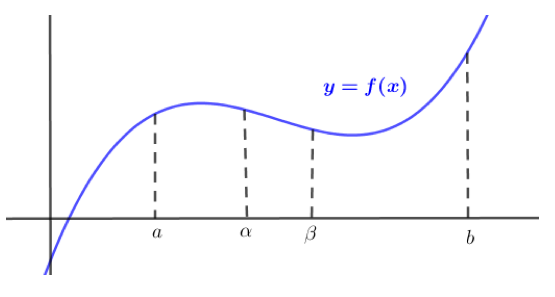
\includegraphics[width=.4\textwidth]{imagenes/imagenes06/T06IM03.png}
		\end{figure}
		\end{multicols}
		
	\begin{equation}
		\label{Taylor}
		\boxed{ \quad P_{n,f,\alpha}(x)=f(\alpha)+\dfrac {f'(\alpha)}{1!} (x-\alpha)+\dfrac {f''(\alpha)}{2!} (x-\alpha)^2+\cdots +\dfrac {f^{n)}(\alpha)}{n!} (x-\alpha)^n \quad}
	\end{equation}
	\centerline{\emph{``Polinomio de Taylor de grado $n$ para $f(x)$ en el punto $x=\alpha$''}}
	
	Para un punto $\beta \in [a,b]$ próximo a $\alpha$, podemos escribir:
	
	$ f(\beta)=f(\alpha)+\dfrac {f'(\alpha)}{1!} (\beta-\alpha)+\dfrac {f''(\alpha)}{2!} (\beta-\alpha)^2+\cdots +\dfrac {f^{n)}(\alpha)}{n!} (\beta-\alpha)^n \; + \; \textbf{E}$
	
	Donde $E$ mide el error cometido al sustituir $f(\beta)$ por $P_{n.f.\alpha}(\beta)$:
	
	$E=f(\beta)- \left[ f(\alpha)+\dfrac {f'(\alpha)}{1!} (\beta-\alpha)+\dfrac {f''(\alpha)}{2!} (\beta-\alpha)^2+\cdots +\dfrac {f^{n)}(\alpha)}{n!} (\beta-\alpha)^n   \right]$, que es el llamado \emph{' término complementario'} y depende de $\alpha$, $\beta$, $n$, incluso, claro está, de $f$.
	
	Supongamos $\beta$ y $n$ fijos y hagamos variar $\alpha$, con ello determinaremos $E(\alpha)$.
	
	$E'(\alpha)=\cancel{-f'(\alpha)}+\cancel{\dfrac{f'(\alpha)}{1!}}-\bcancel{\dfrac {f''(\alpha)}{1!}(\beta-\alpha)} +\bcancel{\dfrac {2f''(\alpha)}{2!}(\beta-\alpha)}-\cdots - \dfrac {f^{n+1)}(\alpha)}{n!}(\beta-\alpha)^n$
	
	
	Luego  $E'(\alpha)=-\dfrac {f^{n+1)(\alpha)}}{n!}(\beta-\alpha)^n$
	
	A partir de esta expresión podemos calcular $E(\alpha)$ aplicando el Teorema \ref{ThCauchy} de Cauchy:
	
	\begin{equation*}
		\dfrac {E(\beta)-E(\alpha)}{\Phi(\beta)-\Phi(\alpha)}=\dfrac {E'(\theta)}{\Phi'(\theta)} \qquad \mbox{ con } \alpha<\theta<\beta
	\end{equation*}
	
	Eligiendo una función $\Phi$ que junto con $E$ cumplan las condiciones del th. de Cauchy.
	
	Como $E(\beta)=0$, elegiremos una $\Phi(x)$ que también se anule en $\beta$. Las más sencillas son: 
	
	$\Phi(x)= (\beta-x)^{n+1}; \quad \Phi(x)= (\beta-x); \quad \Phi(x)= (\beta-x)^p$
	
	Elegimos, es este caso, la primera de las opciones y aplicamos el th. de Cauchy:
	
	\begin{equation*}
		\dfrac{-E(\alpha)}{-(\beta-\alpha)^{n+1}}=\dfrac {-\dfrac {f^{n+1)}(\theta)}{(n+1)!}(\beta-\theta)^n}{-(n+1)(\beta-\theta)^n}
	\end{equation*} 
	
	
	De donde:
	
	\begin{equation}
		E(\alpha)= \dfrac {f^{n+1)}(\theta)}{(n+1)!}\; (\beta-\alpha)^{n+1}
	\end{equation}
	\centerline{\emph{`Forma de \textbf{LAGRANGE} del término complementario'}} 
	\vspace{1mm}
	
	
	Si hubiésemos tomado la segunda opción para $\Phi$, hubiésemos obtenido:
	
	\begin{equation*}
		E(\alpha)=\dfrac {f^{n+1)}(\theta)\; (\beta-\theta)^n}{n!}\; (\beta-\alpha)
	\end{equation*}
	\centerline{\emph{`Forma de CAUCHY del término complementario'}} 
	\vspace{1mm}
	
	Y si hubiésemos elegido la tercera opción:
	
	\begin{equation*}
		E(\alpha)=\dfrac {f^{n+1}(\theta)\; (\beta-\theta)^{n-p+1}}{n! \cdot p}\; (\beta - \alpha)^p
	\end{equation*}
	\centerline{\emph{`Forma de SCHLÖLMILCH del término complementario'}} 
	\vspace{1mm}
	
	Sustituyendo en la fórmula que proporciona $f(\beta)$ se obtiene la '' Fórmula o desarrollo de TAYLOR'' de una función $f(x)$ que admite de derivadas sucesivas. Los términos complementarios expresan el error cometido al aproximar $f(x)$ por $P_n(x)$. En general, el error es mayor cuanto menor es el grado del polinomio y cuanto más alejada esté $x$ de $\alpha$.
	
	El término complementario más usado es el de Lagrange. A estos términos complementarios también se les llama restos.
	
	Haciendo $\beta=x$:
	
	\begin{equation}
		\label{Desarrollo-Taylor}
		\boxed{
		\begin{split}
		\quad f(x)=\left[f(\alpha)+\dfrac {f'(\alpha)}{1!}(x-\alpha)+\dfrac {f''(\alpha)}{2!} (x-\alpha)^2 + \cdots + \dfrac {f^{n}(\alpha)}{n!} (x-\alpha)^n    \right] + \\ 
		+\boxed{\; \dfrac {f^{n+1)}(\theta)}{(n+1)!}\; (x-\alpha)^{n+1}\; } \quad \mbox{con } \alpha < \theta <x .\quad 
		\end{split}
		}
	\end{equation} 
	\centerline{\emph{Desarrollo de Taylor con resto de Lagrange.}} 
		
	El último término del desarrollo es el resto de Lagrange, abreviadamente podríamos escribir:  $f(x)=P_n(x)+E$
	
	Otra forma de escribir este desarrollo es haciendo $x -\alpha=h$:
	
	\begin{equation}
		\label{Desarrollo-Taylor-h}
		\boxed{
		\begin{split}
		\quad f(\alpha+h)=\left[f(\alpha)+\dfrac {f'(\alpha)}{1!}\; h+\dfrac {f''(\alpha)}{2!}\; h^2 + \cdots + \dfrac {f^{n}(\alpha)}{n!} \; h^n    \right]  + \\
		+\boxed{\; \dfrac {f^{n+1)}(\alpha+\theta \cdot h)}{(n+1)!}\; h^{n+1}\; } \quad \mbox{con } 0 < \theta <1 .\quad 
		\end{split}}
	\end{equation}
	
	Al ser $0 < \theta <1 \; $, $\; \alpha+\theta\cdot h$ es un punto intermedio del intervalo de extremos $\alpha$ y $\alpha+h$.
	
	Haciendo $\alpha=0$, tenemos el desarrollo de Maclaurin:
	
	
	\begin{equation}
		\label{Desarrollo-Maclaurin}
		\boxed{
		\begin{split}
		\quad f(x)=\left[f(0)+\dfrac {f'(0)}{1!}\; x+\dfrac {f''(0)}{2!}\; x^2 + \cdots + \dfrac {f^{n}(0)}{n!} \; x^n    \right]  + \\
		+\boxed{\; \dfrac {f^{n+1)}(\theta \; x)}{(n+1)!}\; x^{n+1}\; } \quad \mbox{con } 0 < \theta <1 .\quad 
		\end{split}}
	\end{equation}
	\centerline{\emph{Desarrollo de MacLaurin con resto de Lagrange.}}
	
	
	\section{Aproximaciones locales de algunas funciones}
	
	Recordando los resultados obtenidos en la sección \ref{derivadas-sucesivas} de derivadas sucesivas:
	
	\begin{ejem} Desarrollo de MacLaurin de la función exponencial: $f(x)=e^x$
	
	$n=1 \to e^x=1+	\dfrac {1}{1!}x+ \boxed{\; \dfrac {e^{\theta x}}{2!}x^2}\; $
	
	$n=2 \to e^x=1+	\dfrac {1}{1!}x+ \dfrac {1}{2!}x^2+ \boxed{\; \dfrac {e^{\theta x}}{3!}x^3}\; $
	
	$n=3 \to e^x=1+	\dfrac {1}{1!}x+ \dfrac {1}{2!}x^2+ \dfrac {1}{3!}x^3+\boxed{\; \dfrac {e^{\theta x}}{4!}x^4}\; $
	
	etc $\cdots$
	
	Se dice que $P_1(x)=1+x$ es el polinomio osculatriz de primer grado de o aproximación lineal (\textit{diferencial}) de $e^x$ en el punto $0$; $P_2(x)=1+x+\frac 1 2 x^2$ es el polinomio osculatriz de segundo grado de o aproximación cuadrática  de $e^x$ en el punto $0$; $P_3(x)=1+x+\frac 1 2 x^2+ \frac 1 6 x^3$ es el polinomio osculatriz de tercer grado de o aproximación cúbica  de $e^x$ en el punto $0$;	$\cdots$
	
	Esquemáticamente:  
	\begin{equation}\label{MacLaurin-exp}
		\boxed{\quad { e }^{ x }\; =\; \sum _{ k=1 }^{ n }{ \dfrac { 1 }{ k! } \; { x }^{ k } } 	\quad +\quad \dfrac { { e }^{ \theta x } }{ (k+1)! } { x }^{ k+1 } \quad}  
	\end{equation}
	\centerline{\emph{Desarrollo de MacLaurin de $e^x$.}}
	
	Como ejercicio, vamos a calcular con aproximación lineal, cuadrática y cúbica, el valor aproximado que da el desarrolla para $e^{0.4}$, así como intentar acotar los errores cometidos.
	
	\vspace{2mm}
	
	$n=1 \to e^{0.4}=1+0.4=1.4 $. Aproximación lineal.
	
	$E=\dfrac {e^{\theta x}}{2!}\; (0.4)^2 < dfrac {e^1}{2}\; 0,16 < \dfrac {3}{2} \cdot (0.16)=0.24 \qquad 0<\theta x< 0,4$
	
	\vspace{2mm}
	
	$n=2 \to e^{0.4}=1+0.4+\frac 1 2\;  0.4^2=1.48 $. Aproximación cuadrática.
	
	$E=\dfrac {e^{\theta x}}{3!}\; (0.4)^3 < dfrac {e^1}{6}\; 0,064 < \dfrac {3}{6} \cdot (0.064)=0.24 \qquad 0<\theta x< 0,032$
	
	
	\begin{multicols}{2}

	$\quad$
	
	$n=2 \to e^{0.4}=1+0.4+\frac 1 2 \; 0.4^2+ \frac 1 {6}\; 0.4^3 =1.490666\cdots $. Aproximación cúbica.
	
	$E=\dfrac {e^{\theta x}}{4!}\; (0.4)^4 < \dfrac {e^1}{24}\; 0,0256 < \dfrac {3}{24} \cdot (0.0256)=0.24 \qquad 0<\theta x< 0,0032$
	
	$\quad$
	
	Mostramos una figura que represente $e^x$ y las sucesivas aproximaciones $ P_1; P_2; P_3$
	
	\begin{figure}[H]
	\centering
		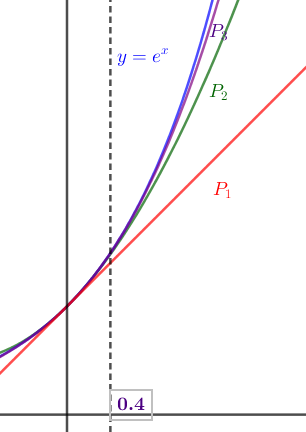
\includegraphics[width=.3\textwidth]{imagenes/imagenes06/T06IM04.png}
		\end{figure}
	\end{multicols}
	\end{ejem}
	 
	 \begin{ejem}  Desarrollo de MacLaurin de la función seno: $f(x)=\sin x$
	 
	 En la sección \ref{derivadas-sucesivas} vimos que $\sin^{n)}(x)=\sin (x+n\frac \pi 2)$
	 
	 En $x=0$, para $n=0\to \sin 0=0; \quad n=1\to \sin (\pi/2)=1; \quad n=2\to \sin (2\pi/2)=\sin (\pi)=0; \quad n=3 \to \sin (3\pi/2)=-1; \quad \cdots $. Solo quedan las derivadas impares.
	 
	 El desarrollo de MacLaurin, hasta orden 6 (desarrollar hasta orden 5 es tontería, ya que el término de orden 6 es par, cero. De este modo, el error cometido se medirá con el término séptimo y nos dará más precisión). ¡OJO, $x$ en radianes!
	 
	 $\sin x= \dfrac {1}{1!}x-\dfrac {1}{3!}x^3+\dfrac {1}{5!}x^5 +\dfrac {\sin \theta x}{7!}x^7; \quad 0<\theta <x$
	 
	 
	 Calculemos una aproximación de quinto grado del $\sin(0.2)$, así como una cota del error cometido:
	 
	 
	  $\sin 0.2= \dfrac {1}{1!}0.2-\dfrac {1}{3!}0.2^3+\dfrac {1}{5!}0.2^5=1.988669333\cdots$

	  Acotemos el error: $|E|=\left| \dfrac {\sin (\theta x)}{7!} \right|\; 0.2^7 < \; [\; \sin (\theta x) < 1 \;] < 0,000000002539683 < 0,0000000026 $
	  
	  Adjuntamos una imagen al ejemplo.
	  
	\begin{figure}[H]
	\centering
		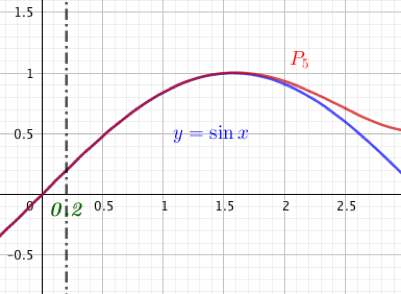
\includegraphics[width=.6\textwidth]{imagenes/imagenes06/T06IM05.png}
	\end{figure}
	
	El desarrollo completo de la función $\sin x$ es:
	
	$\sin x \approx x-\dfrac{x^3}{3!}+\dfrac{x^5}{5!}-\dfrac{x^7}{7!}+\cdots$. Escrito más brevemente e incluyendo el resto de Lagrange:
	
	\begin{equation}\label{MacLaurin-exp}
		\boxed{\quad \sin x \; =\; \sum _{ k=1 }^{ n }{ \dfrac {(-1)^k}{(2k+1)!}\;x^{2k+1}  +\dfrac {(1)^{2k+3}}{(2k+3)!} \; x^{2k+3}\quad}}  
	\end{equation}
	\centerline{\emph{Desarrollo de MacLaurin de $\sin x$.}}
	
	\end{ejem}
	
	\begin{ejem}Desarrollo de Taylor para de la función logarítmica  $f(x)=\mathrm{ln}\;x$, en un entorno de $\alpha=e$:
	
	$\mathrm{ln}\; x = 1 + \dfrac 1 1 \dfrac 1 e (x-e) +- \dfrac 1 2 \dfrac 1 {e^2} (x-e)^2 + \cdots + \dfrac {(-1)^{n-1}}{n} \dfrac 1 {e^n} (x-e)^n + $
	
	$ + \dfrac {(-1)^n}{n+1} \dfrac 1 {\theta ^{n+1}} (x-e)^{n+1} \qquad e < \theta < x \quad \vee \quad 0 < x < \theta < e$
	
	Como aplicación, calcularemos un polinomio de tercer grado osculatriz para aproximar $\mathrm{ln}\; 3$ y una cota del error cometido.
	
	$\mathrm{ln}\; 3 = 1+ \frac 1 e 3-e)- \frac 1 {2e^2}(3-x)^2+ \frac 1 {3e^3}(3-e=^3 = 1.09861$
	
	$|E|=|\; - \frac 1 4 \frac 1 {\theta^4} (3-e)^4  \;| < 0.00004; \quad (e<\theta<3) \;$
		
	\end{ejem}
	
	En el apartado de Apéndices, \ref{tabla-maclaurin},  aparecerá una relación de los desarrollos de MacLaurin más usados, así como sus `radios de convergencia'.
	
	\section{Aplicaciones de la fórmula de Taylor}
	
	\subsection{Determinación de máximos y mínimos}
	
	Sabemos, por la observación del teorema \ref{CS-extremos}, que la condición necesaria para que una función $y=f(x)$ tenga en extremos relativo en $x=c$ es que $f'(c)=0$. 
	 
	 También, por el teorema \ref{teor-crit-deriv2} criterio de la segunda derivada, sabemos que si $f'(c)=0\; \vee \ \; f''(c)=0$, tenemos dudas y no podemos asegurar nada (solo que en $x=c$ la tangente es horizontal, pero podría tratarse de un extremo o de una inflexión).
	 
	 Vamos a desarrollar un método que resolverá todos los posibles casos que se presenten basado en el desarrollo de Taylor con resto de Lagrange de $f(x)$.
	 
	 \vspace{2mm}
	 
	 Sea $y=f(x)$, definida y derivable hasta orden $n$ en $[a,b]$, tal que $f^{n)}(x)$ sea continua en $[a,b]$ y derivable en $]a,b[$. Admitimos. además, que en un punto $x=c$ se cumple que $f'(c)=f''(c)=f'''(c)=\cdots = f^{n)}(c)=0$, con $a<c<b$
	 
	 Usando la fórmula de Taylor con resto de Lagrange, ecuación \ref{Desarrollo-Taylor-h}:
	 
	 $f(c+h)=f(c)+0+0+0+\cdots+0+\dfrac {f^{n+1)}(c+\theta h)}{(n+1)!} h^{n+1}$ 
	 
	 Distinguiremos ahora dos casos, según sea $n+1=m$ par o impar \emph{($m$ es el índice de la primera derivada que no es nula en  $x=c$)}:
	 
	 \begin{itemize}
	 	\item Si m es par: al pasar $h$ de valores negativos a positivos, $h^{n+1}=h^m$ no cambia de signo, mientras que la derivada $f^{n+1)}(c+\theta h)$ conserva el mismo signo que en el punto $c$ por ser $f^{n+1)}(x)$ continua (teorema \ref{teor:conserva-signo} de la conservación del signo). Si $|h|$ es menor que cierto $\delta>0$, entonces, el incremento de la función conserva el mismo signo que la derivada $f^{n+1)}(c)$, luego como $|h|< \delta$ :
	 	
	 	$\circ \quad$ si $f^{n+1)}(c)<0 \to f(c-h)<f(c)>f(c+h) \to c\; $ máximo
	 	
	 	$\circ \quad$ si $f^{n+1)}(c)>0 \to f(c-h)>f(c)<f(c+h) \to c\; $ mínimo.

	\vspace{2mm}CONCLUSIÓN-1: La `condición necesaria y suficiente` para que $y=f(x)$ que admite derivadas sucesivas hasta orden $n$ en $[a,b]$ y tal que $f^{m)}(x)$ es continua en $[a,b]$ y derivable en $]a,b[$ tenga en un punto $c \in [a,b]$ un extremo (máximo o mínimo) relativo es que la primera derivada que no se anule en $x=c$ sea de orden par. Si esta derivada es negativa, en $c$ habrá un máximo relativo y, si es positiva, en $c$ habrá un mínimo.
	
	\item Si m es impar: al pasar $h$ de valores negativos a positivos, $h^{n+1}=h^m$ si cambia de signo, mientras que la derivada $f^{n+1)}(c+\theta h)$ conserva el mismo signo que en el punto $c$ por ser $f^{n+1)}(x)$ continua (teorema \ref{teor:conserva-signo} de la conservación del signo). Si $|h|$ es menor que cierto $\delta>0$, entonces, el incremento de la función conserva el mismo signo que la derivada $f^{n+1)}(c)$, luego como $|h|< \delta$ :
	 
	
	 $\circ \qquad  f(c-h)<f(c)<f(c+h) \quad \wedge \quad f(c-h)>f(c)>f(c+h)$	
	 
	 La curva queda atravesada por la tangente y en $c$ tenemos un punto de inflexión de tangente horizontal ($f'(c)=0$).
	 
	 \vspace{2mm}CONCLUSIÓN-2: La `condición necesaria y suficiente` para que $y=f(x)$ que admite derivadas sucesivas hasta orden $n$ en $[a,b]$ y tal que $f{m)}(x)$ es continua en $[a,b]$ y derivable en $]a,b[$ tenga en un punto $c \in [a,b]$ un punto de inflexión  (de tangente horizontal: $f'(c)=0$) es que la primera derivada que no se anule en $x=c$ sea de orden impar. 
	 
	 \end{itemize}
	 
	 
	\begin{ejem}
		Hallar los extremos relativos de la función 
		
		$f(x)=(x^2-3x+2)^4$	
			
		$f'(x)=4(x^2-3x+2)^3(2x-3)=0 \leftrightarrow x=3/2 \; \wedge \; x=1 \; \wedge \; x=2 $
		   
		$f'(3/2)=0; \; f''(3/2)<0 \to x=3/2\; $ máximo local
		
		$f'(1)=f''(1)=f'''(1)=0; \; y^{iv}(1)>0 \to x=1\; $ mínimo local
		
		$f'(2)=f''(2)=f'''(2)=0; \; y^{iv}(2)<0 \to x=1\; $ máximo local
		
	\end{ejem}
	
	\begin{ejem} Encuentra los PI de $y=(x+3)^5$
	
	$y'=5(x+3)^4=0 \leftrightarrow x=-3$
	
	$y'(-3)=y''(-3)=y'''(-3)=y^{iv}(-3)=0; \; y^{v}{-3}=5!>0 \to x=-3\; $ P.I.
	
	\end{ejem}
	
	\subsection{Aplicaciones de la fórmula de Taylor al cálculo de límites}

	Si es posible, se bebe sustituir cada expresión de la expresión cuyo límite se desea calcular por el desarrollo adecuado de Taylor. El problema del cálculo de límites se reduce al problema del cálculo de límites de funciones polinómicas.
	
	\begin{ejem}
	Calcula $\quad \underset{x\to 0}{lim}\;{\dfrac {\tan 2x - 2 \tan x}{x \; \tan x \; \tan 2x}}$	
	
	MacLaurin: (Apéndice \ref{tabla-maclaurin})
	
	$\tan x=x+x^3/3+ \cdots$
	
	$\tan 2x = 2x + (2x)^3/3 + \cdots = 2x + \frac 8 3 x^3 + \cdots $
	
	Sustituyendo:
	
	$\underset{x\to 0}{lim}\;{\dfrac {\tan 2x - 2 \tan x}{x \; \tan x \; \tan 2x}}= \underset{x\to 0}{lim}\; { \dfrac {  (2x + \frac 8 3 x^3 + \cdots ) - 2\; (x+x^3/3+ \cdots) }  {  x\cdot (x+x^3/3+ \cdots) \cdot(2x + \frac 8 3 x^3 + \cdots )   }    } =$
	
	$ = \underset{x\to 0}{lim}\;{\dfrac {2x^3+\cdots}{2x^3+\cdots}}=1$ 
	
	$\quad$
	
	Compare el lector la rapidez del cálculo por este método o aplicando la regla de L'Hôpital.

	\end{ejem}
	
	\begin{ejem} Calcula $\underset{x\to 0}{lim}\;{\dfrac {\tan x \; \arctan x- x^2}{x^6}}$
	
	Se necesita derivar al menos 5 veces (L'H) numerador y denominador para resolver el límite.
	
	Si sustituimos las expresiones por los desarrollos de MacLaurin (Apéndice \ref{tabla-maclaurin}) y hacemos cuatro operaciones con los polinomios, tendremos:
	
	$\underset{x\to 0}{lim}\;{\dfrac {\tan x \; \arctan x- x^2}{x^6}}= \underset{x\to 0}{lim}{\dfrac {\frac 2 9 \; x^6 + \cdots }{x^6}}\;=2/9$
	
	\end{ejem}
	



\section{Ejercicios resueltos}

	\begin{ejre} Calcula $\underset{x\to 0}{lim}\;{\dfrac {(\cos x -1)(\mathrm{ln}((1+x)-x)-\frac 1 4 x^4}{x^5}}$
		
	\end{ejre}

	\begin{proofw}\renewcommand{\qedsymbol}{$\diamond$}	

	Acudiendo al apéndice\ref{tabla-maclaurin} de los desarrollos de MacLaurin:
	
	$\underset{x\to 0}{lim}\;{\dfrac {(\cos x -1)(\mathrm{ln}((1+x)-x)-\frac 1 4 x^4}{x^5}} = -1/6$
	\end{proofw}

	\begin{ejre} Sea $f(x)=e^{2x}$. En contrar el órden $n$ del polinomio de Taylor de$f$ en $x_0=0$ (MacLaurin) tal que al aproximar $f(1)=e^2$ por el $P_n$ encontrado, el error sea menor que $\dfrac 1 {1000}$ (una milésima).
		
	\end{ejre}
	
	\begin{proofw}\renewcommand{\qedsymbol}{$\diamond$}	
		
		$f'(x)=2e^{2x}; \; f''(x)=2^2 e^{2x}; \; f'''(x)=2^3 e^{2x}; \cdots ; \; f^{n)}(x)=2^n e^{2x}$
		
		Por ello:
		
		$f(0)=1; \; f'(0)=2; \; f''(2)=2^2; \; f'''(2)=2^3; \cdots ; \; f^{n)}(0)=2^n$
		
		El polinomio de MacLaurin de orden $n$ es:
		
		$P_n(x)=1+ 2x+\dfrac{4}{2}x^2+\dfrac{8}{6}x^3+ \cdots + \dfrac{2^n}{n!}x^n$
		
		Vamos a por el resto de Lagrange:
		
		$E_n(x)=\dfrac{2^{n+1}\; e^{2\theta}}{(n+1)!}\; x^{n+1}$
		
		Como $\theta\in]0,x[$, con $x>0$, tenemos: (queremos calcular $f(1); \quad \theta=1$)
		
		
		$E_n(1)=\dfrac{2^{n+1}\; e^{2 \theta}}{(n+1)!}\; 1^{n+1} < 
		\dfrac{2^{n+1}\; e^{2\cdot 1}}{(n+1)!}\; 1^{n+1} <
		 \dfrac{2^{n+1}\; 3^{2}}{(n+1)!} < \dfrac {18\cdot 2^n}{(n+1)!} < \dfrac {1}{100}  $
		
		
		La última ecuación $\dfrac {18\cdot 2^n}{(n+1)!} < \dfrac {1}{100}  $, que nos sirve para determinar el grado $n$ que hemos de tomar para aproximar $f(1)$ por $P_n(1)$ solo puede ser resuelta por `tanteo'. Probando, encontramos:
		
		$E_{10}(1)<\dfrac {2^{10+1}3^2}{(10+1)!}=\dfrac {8}{17325}\approx 0.00046\cdots < \dfrac {1}{1000}$
		
		Puede el lector calcular $P_{10}(1)$ y comparar (con una calculadora) con el valor de f(1) para comprobar que el error que se comete es, efectivamente, menor que una milésima.

	\end{proofw}

	\begin{ejre} Probar que $\quad \forall \; x \; \in \; \mathbb{R}\; : \quad e^x \; \ge \; 1 + x$
		
	\end{ejre}
	\vspace{-3mm}
	\begin{proofw}\renewcommand{\qedsymbol}{$\diamond$}	
		Acudiendo al desarrollo es serie de MacLaurin de la función $e^x$:
		
		$e^x=1+x+E\ge 1+x \qquad \mbox{ ya que } \quad E=\dfrac {e^c}{2!}x^2\ge 0$
	\end{proofw}

	
	

	 	
	

	
